\documentclass[UTF8, 12pt]{ctexart}
% UTF8编码,ctexart现实中文
\usepackage{xcolor}
% 使用颜色
\definecolor{orange}{RGB}{255,127,0} 
\definecolor{violet}{RGB}{192,0,255} 
\definecolor{aqua}{RGB}{0,255,255} 
\usepackage{geometry}
\setcounter{tocdepth}{4}
\setcounter{secnumdepth}{4}
% 设置四级目录与标题
\geometry{papersize={21cm,29.7cm}}
% 默认大小为A4
\geometry{left=3.18cm,right=3.18cm,top=2.54cm,bottom=2.54cm}
% 默认页边距为1英尺与1.25英尺
\usepackage{indentfirst}
\setlength{\parindent}{2.45em}
% 首行缩进2个中文字符
\usepackage{amssymb}
% 因为所以与其他数学拓展
\usepackage{amsmath}
% 数学公式
\usepackage[colorlinks,linkcolor=black,urlcolor=blue]{hyperref}
% 超链接
\usepackage{setspace}
\renewcommand{\baselinestretch}{1.5}
% 1.5倍行距
\usepackage{pifont}
% 圆圈序号
\usepackage{tikz}
% 绘图
\usepackage{array}
% 设置表格行距
\author{Didnelpsun}
\title{导数与微分}
\date{}
\begin{document}
\renewcommand{\arraystretch}{1.5}
% 表格高1.5倍
\maketitle
\thispagestyle{empty}
\tableofcontents
\thispagestyle{empty}
\newpage
\pagestyle{plain}
\setcounter{page}{1}
\section{导数概念}
\subsection{引例}

设$f(x)$下$x$在$x_0$的邻域内,$\alpha$为切线所成夹角。

$\tan\alpha=f'(x_0)=\lim\limits_{x\to x_0}\dfrac{f(x)-f(x_0)}{x-x_0}=k$。

导数的本质是增量比的极限。

\subsection{定义}

设$y=f(x)$定义在区间$I$上,让自变量在$x=x_0$处加一个增量$\Delta x$,其中$x_0\in I$,$x_0+\Delta x\in I$,则可得函数的增量$\Delta y=f(x_0+\Delta x)-f(x_0)$。若函数增量$\Delta y$与自变量增量$\Delta x$的比值在$\Delta x\to 0$时的极限存在,则称函数$y=f(x)$在$x_0$处可导,并称这个极限为$y=f(x)$在点$x_0$处的导数,记作$f'(x)$,即$f'(x)=\lim\limits_{\Delta x\to 0}\dfrac{\Delta y}{\Delta x}=\lim\limits_{\Delta x\to 0}\dfrac{f(x_0+\Delta x)-f(x_0)}{\Delta x}$。\medskip

下面三句话等价:

\begin{enumerate}
    \item $y=f(x)$在$x_0$处可导。
    \item $y=f(x)$在$x_0$处导数存在。
    \item $f'(x)=A$。($A$为有限数)
\end{enumerate}

单侧导数分为左导数和右导数。\medskip

$f'_-(x)=\lim\limits_{\Delta x\to 0^-}\dfrac{\Delta y}{\Delta x}=\lim\limits_{\Delta x\to 0}\dfrac{f(x_0+\Delta x)-f(x_0)}{\Delta x}$

$f'_+(x)=\lim\limits_{\Delta x\to 0^+}\dfrac{\Delta y}{\Delta x}=\lim\limits_{\Delta x\to 0}\dfrac{f(x_0+\Delta x)-f(x_0)}{\Delta x}$\medskip

所以$f(x)$在$x_0$处可导的充要条件是其左导数和右导数存在且相等。

若$f(x)$在$x_0$的左右,如$y=\vert x\vert$在$0$的左右出现了单侧的不同的切线,那这个$x_0$就是一个\textbf{角点},该角点处不可导。

若$f(x)$在$x_0$处导数为无穷,如$y=x^{\frac{1}{3}}$在$0$处利用导数的极限定义计算得到为正无穷,那么该点的导数为无穷导数,在考研中被认为是不存在的。

\textbf{例题:}证明若$f(x)$为可导的偶函数,则$f'(x)$为奇函数,若$f(x)$为可导的奇函数,则$f'(x)$为偶函数。

该证明是准备部分的定理。

首先已知$f(-x)=f(x)$,证明$f'(-x)=-f'(x)$。

$\therefore$

$
\begin{aligned}
    f'(-x) &=\lim\limits_{\Delta x\to 0}\dfrac{f(-x+\Delta x)-f(-x)}{\Delta x} \\
    & =\lim\limits_{\Delta x\to 0}\dfrac{f(x+(-\Delta x))}{\Delta x} \\
    & =-\lim\limits_{-\Delta x\to 0}\dfrac{f(x+(-\Delta x))}{-\Delta x} \\
    & =-f'(x)
\end{aligned}
$

同理得证$f(-x)=-f(x)\Rightarrow f'(-x)=f'(x)$。

\textbf{例题:}证明$f(x)$为可导的周期为$T$的周期函数,则$f'(x)$也是以$T$为周期的周期函数。

已知$f(x+T)=f(x)$,求证$f'(x+T)=f'(x)$。\medskip

$\therefore f'(x+T)=\lim\limits_{\Delta x\to 0}\dfrac{f(x+T+\Delta x)-f(x+T)}{\Delta x}$

$=\lim\limits_{\Delta x\to 0}\dfrac{f(x+\Delta x)-f(x)}{\Delta x}=f'(x)$。

\textbf{例题:}设$f(x)$是二阶可导的以2为周期的奇函数,且$f(\dfrac{1}{2})>0$,$f'(\dfrac{1}{2})>0$,比较$f(-\dfrac{1}{2})$、$f'(\dfrac{3}{2})$、$f''(0)$的大小。\medskip

$\because f(x)$为二阶奇函数,$\therefore f(x)\text{奇函数}\Rightarrow f'(x)\text{偶函数}\Rightarrow f''(x)\text{奇函数}\Rightarrow f''(0)=0$。

$\therefore f(-\dfrac{1}{2})=-f(\dfrac{1}{2})<0$。

$\because f(x)T=2\Rightarrow f'(x)T=2$,$\therefore f'(\dfrac{3}{2})=f'(\dfrac{3}{2}-2)=f'(-\dfrac{1}{2})=f'(\dfrac{1}{2})>0$。

$\therefore f'(\dfrac{3}{2})>f''(0)>f(-\dfrac{1}{2})$。\medskip

\textbf{例题:}$\left(x^\alpha\right)'=\alpha x^{\alpha-1}(x>0)$。\medskip

$\lim\limits_{\Delta x\to 0}\dfrac{f(x+\Delta x)-f(x)}{\Delta x}$\medskip

$=\lim\limits_{\Delta x\to 0}\dfrac{\left(x+\Delta x\right)^\alpha-x^\alpha}{\Delta x}$\medskip

$=\lim\limits_{\Delta x\to 0}\dfrac{x^\alpha\left[\left(1+\dfrac{\Delta x}{x}\right)^\alpha-1\right]}{\Delta x}$\medskip

$=\lim\limits_{\Delta x\to 0}\dfrac{x^\alpha\cdot\alpha\cdot\dfrac{\Delta x}{x}}{\Delta x}$\medskip

$=\alpha x^{\alpha-1}$

\subsection{导数的几何意义}

导数$f'(x_0)$在几何上就是曲线$y=f(x)$在点$(x_0,f(x_0))$处切线的斜率。

切线方程:$y-y_0=f'(x_0)(x-x_0)$。

法线方程:$y-y_0=-\dfrac{1}{f'(x_0)}(x-x_0)$。

\subsection{可导与连续的关系}

可导必连续,连续不一定可导。

\textbf{例题:}证明可导必连续。

已知连续定义:$\lim\limits_{\Delta x\to 0}f(x+\Delta x)=f(x)$,即$\lim\limits_{\Delta x\to 0}f(x+\Delta x)-f(x)=0$。

可导定义:$f'(x)=\lim\limits_{\Delta x\to 0}\dfrac{f(x+\Delta x)-f(x)}{\Delta x} = A$

$\lim\limits_{\Delta x\to 0}f(x+\Delta x)-f(x)$

$=\lim\limits_{\Delta x\to 0}\dfrac{f(x+\Delta x)-f(x)}{\Delta x}\cdot\Delta x$

$=A\cdot 0$

$=0$

\textbf{例题:}若$f(x)$在$x=x_0$处连续,且$\lim\limits_{x\to x_0}\dfrac{f(x)}{x-x_0}=A$,则$f(x_0)=0$且$f'(x_0)=A$。

证明:$\because\text{连续,}\therefore f(x_0)=\lim\limits_{x\to x_0}f(x)=\lim\limits_{x\to x_0}\dfrac{f(x)}{x-x_0}(x-x_0)=A\cdot 0=0$。

又$f'(x_0)=\lim\limits_{x\to x_0}\dfrac{f(x)-f(x_0)}{x-x_0}=\lim\limits_{x\to x_0}\dfrac{f(x)}{x-x_0}=A$。

如$\lim\limits_{x\to 1}\dfrac{f(x)}{x-1}=2$且$f(x)$连续,可以推出$f(1)=0$与$f'(1)=2$。


\section{函数求导法则}

\subsection{四则运算}

若函数可导:

\begin{enumerate}
    \item 和差的导数:$[u(x)\pm v(x)]'=u'(x)\pm v'(x)$。
    \item 积的导数:$[u(x)v(x)]'=u'(x)v(x)+u(x)v'(x)$,\\ $[u(x)v(x)w(x)]'=u'(x)v(x)w(x)+u(x)v'(x)w(x)+u(x)v(x)+w'(x)$。
    \item 商的导数:$\left[\dfrac{u(x)}{v(x)}\right]'=\dfrac{u'(x)v(x)-u(x)v'(x)}{[v(x)]^2}$,$v(x)\neq 0$。
\end{enumerate}

\textbf{例题:}证明$(uv)'=u'v+uv'$。

令$f(x)=u(x)v(x)$。

$(u\cdot v)'$

$=f'(x)$

$=\lim\limits_{\Delta x\to 0}\dfrac{f(x+\Delta x)-f(x)}{\Delta x}$

$=\lim\limits_{\Delta x\to 0}\dfrac{u(x+\Delta x)v(x+\Delta x)-u(x)v(x)}{\Delta x}$

$=\lim\limits_{\Delta x\to 0}\dfrac{u(x+\Delta x)v(x+\Delta x)-u(x)v(x+\Delta x)+u(x)v(x+\Delta x)-u(x)v(x)}{\Delta x}$

$=\lim\limits_{\Delta x\to 0}\dfrac{u(x+\Delta x)-u(x)}{\Delta x}v(x+\Delta x) +\lim\limits_{\Delta x\to 0}\dfrac{v(x+\Delta x)-v(x)}{\Delta x}u(x)$

$=u'(x)v(x)+v'(x)u(x)$

\subsection{反函数导数}

\textcolor{aqua}{\textbf{定理:}}$y=f(x)$可导,且$f'(x)\neq 0$,则存在反函数$x=\varphi(y)$,且$\dfrac{\rm{d}x}{\rm{d}y}=\dfrac{1}{\dfrac{\rm{d}y}{\rm{d}x}}$,即$\varphi'(x)=\dfrac{1}{f'(x)}$。\medskip

$y=f(x)$可导,且$f'(x)\neq 0$就是指严格单调,而严格单调必有反函数。

\textbf{例题:}求$y=\arcsin x,x\in(-1,1)$与$y=\arctan x$的导数。

首先反三角函数就是三角函数的反函数。

求$y=\arcsin x$,即$x=\sin y$。

$\therefore\dfrac{\rm{d}\arcsin x}{\rm{d}x}=\dfrac{1}{\dfrac{\rm{d}\sin y}{\rm{d}y}}=\dfrac{1}{\cos y}=\dfrac{1}{\sqrt{1-\sin^2y}}=\dfrac{1}{\sqrt{1-x^2}}$。\medskip

求$y=\arctan x$,就$x=\tan y$。\medskip

$\therefore\dfrac{\rm{d}\arctan x}{\rm{d}x}=\dfrac{1}{\dfrac{\rm{d}\tan y}{\rm{d}y}}=\dfrac{1}{\sec^2y}=\dfrac{1}{1+\tan^2y}=\dfrac{1}{1+x^2}$。\medskip

二阶反函数导数\textcolor{aqua}{\textbf{定理:}}:

$f''(x)$

$=y''_{xx}$\medskip

$=\dfrac{\rm{d}\left(\dfrac{\rm{d}y}{\rm{d}x}\right)}{\rm{d}x}$\medskip

$=\dfrac{\rm{d}^2y}{\rm{d}x^2}$\medskip

$=\dfrac{\rm{d}\left(\dfrac{1}{\varphi'(y)}\right)}{\rm{d}x}$\medskip

$=\dfrac{\rm{d}\left(\dfrac{1}{\varphi'(y)}\right)}{\rm{d}y}\cdot\dfrac{\rm{d}y}{\rm{d}x}$\medskip

$=-\dfrac{x_{yy}''}{(x_y')^2}\cdot\dfrac{1}{x_y'}$\medskip

$=-\dfrac{x_{yy}''}{(x_y')^3}$\medskip

其中$\rm{d}x\cdot\rm{d}x=(\rm{d}x)^2=\rm{d}x^2$称为微分的幂,而$\rm{d}(x^2)$叫幂的微分。

\textbf{例题:}设$y=f(x)$的反函数是$x=\varphi(y)$,且$f(x)=\int_1^{2x}e^{t^2}\rm{d}t+1$,求$\varphi''(1)$。

$\because y=f(x)$,$\therefore x=\varphi(y)$,$x_{yy}''=\varphi''(y)=-\dfrac{y_{xx}''}{(y_x')^3}=-\dfrac{f''(x)}{[f'(x)]^3}$。\medskip

其中根据变限积分求导公式:$f'(x)=2e^{4x^2}$,$f''(x)=2e^{4x^2}\cdot 8x=16xe^{4x^2}$。\medskip

又$y=1\Rightarrow x=\dfrac{1}{2}\Rightarrow\varphi''(1)=-\dfrac{f''\left(\dfrac{1}{2}\right)}{\left[f'\left(\dfrac{1}{2}\right)\right]^3}=-\dfrac{1}{e^2}$。

\subsection{复合函数的导数}

$u=g(x)$在$x$可导,$y=f(u)$在$u=g(x)$处可导,则$\{f[g(x)]\}'=f'[g(x)]g'(x)$。

\textbf{例题:}设$f(x)=\Pi_{n=1}^{100}\left(\tan\dfrac{\pi x^a}{4}-n\right)$,则$f'(1)$为?

原式=$\left(\tan\dfrac{\pi x}{4}-1\right)\left(\tan\dfrac{\pi x^2}{4}-2\right)\cdots\left(\tan\dfrac{\pi x^100}{4}-100\right)$。

令$\left(\tan\dfrac{\pi x^2}{4}-2\right)\cdots\left(\tan\dfrac{\pi x^100}{4}-100\right)=g(x)$。\medskip

$\therefore f(x)=\left(\tan\dfrac{\pi x}{4}-1\right)\cdot g(x)$。\medskip

$\therefore f'(x)=\sec^2\dfrac{\pi x}{4}\cdot\dfrac{\pi}{4}\cdot g(x)+\left(\tan\dfrac{\pi x}{4}-1\right)\cdot g'(x)$。\medskip

$\therefore$根据导数的四则运算,需要导数的乘积为每一项求导乘以其他不求导项的和,而$\tan\dfrac{\pi x}{4}-1$当$x=1$时为0,只要它不求导,其他的项都必然是0,所以原式的后面的结果都是0。

$\therefore$

$f'(1)$

$=f'(x)\vert_{x=1}$\medskip

$=\dfrac{\pi}{2}\cdot g(1)+0\cdot g'(x)$\medskip

$=\dfrac{\pi}{2}\cdot g(1)$\medskip

$=\dfrac{\pi}{2}(-1)(-2)\cdots(-99)$

$=-\dfrac{\pi}{2}\cdot 99!$

\subsection{分段函数的导数}

设$f(x)=\left\{
    \begin{array}{lcl}
        f_1(x), & & x\geqslant x_0 \\
        f_2(x), & & x<x_0 \\
    \end{array}
\right.$。\medskip

在分段点用定义:

判断$f'_+(x_0)=\lim\limits_{x\to x_0^+}\dfrac{f_1(x)-f(x_0)}{x-x_0}\overset{?}{=}\lim\limits_{x\to x_0^-}\dfrac{f_2(x)-f(x_0)}{x-x_0}$。如果相等就挖去这个点,否则就包含这个点。

非分段点使用导数公式求导:$x>x_0,f'(x)=f_1'(x),x<0,f'(x)=f_2'(x)$。

\subsection{对数求导法}

对于多项相乘、相除、开方、乘方的式子,一般先取对数再求导,设$y=f(x)(f(x)>0)$,则\ding{172}等式两边取对数:$\ln y=\ln f(x)$。\ding{173}两边对自变量$x$求导,得$\dfrac{1}{y}y'=[\ln f(x)]'\Rightarrow y'=y[\ln f(x)]'$。

\textbf{例题:}求$y=\sqrt[3]{\dfrac{(x+1)(2x-1)^2}{(4-3x)^5}}$的导数。

取对数:$\ln\vert y\vert=\dfrac{1}{3}[\ln\vert x+1\vert+2\ln\vert 2x-1\vert-5\ln\vert 4-3x\vert]$。

$\because \ln\vert y\vert'=\ln y'$。

两边对x求导:\medskip

$\dfrac{y'}{y}=\dfrac{1}{3}\left(\dfrac{1}{x+1}+\dfrac{4}{2x-1}-\dfrac{5}{4-3x}\cdot(-3)\right)$

$\therefore y'=\dfrac{1}{3}\left(\dfrac{1}{x+1}+\dfrac{4}{2x-1}-\dfrac{5}{4-3x}\cdot(-3)\right)y$

\subsection{幂指函数求导法}

非常重要。

对于$u(x)^{v(x)}(u(x)>0,u(x)\neq 1)$,除了对数求导法外还可以使用指数函数$u(x)^{v(x)}=e^{v(x)\ln u(x)}$。

然后求导得到$[u(x)^{v(x)}]'$$=[e^{v(x)\ln u(x)}]'$

$=u(x)^{v(x)}\left[v'(x)\ln u(x)+v(x)\cdot\dfrac{u'(x)}{u(x)}\right]$。

\textbf{例题:}求$y=x^x(x>0)$的导数。

$\because x^x=e^{x\ln x}$,$\therefore (x^x)'=(e^{x\ln x})'=x^x\cdot(\ln x+1)$。

\textbf{例题:}求解$y=x^{\frac{1}{x}}(x>0)$的整数最大值。

$\because y=x^{\frac{1}{x}}=e^{\frac{1}{x}\ln x}$。

$\therefore y'=\left(x^{\frac{1}{x}}\right)=\left(e^{\frac{1}{x}\ln x}\right)'=x^{\frac{1}{x}}\cdot\dfrac{1-\ln x}{x^2}$。

令导数结果为0,因为$x^{\frac{1}{x}}$与$x^2$在$x>0$时都不为0,所以只有一个驻点$x=e$。

$0<x<e$时$1-\ln x$大于0,所以导数大于0,函数在该区间增。相反$x>e$时函数在区间减。

研究驻点左侧情况,求对应的极限:$e^{\lim\limits_{x\to 0^+}\frac{\ln x}{x}}=e^{-\infty}\to 0$。

研究驻点右侧情况,求对应的极限:$e^{\lim\limits_{x\to+\infty}\frac{\ln x}{x}}=e^0\to 1$。

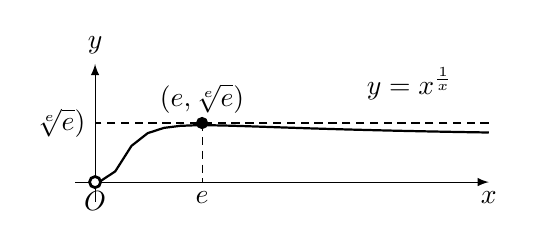
\begin{tikzpicture}[scale=0.5]
    \draw[-latex](-0.5,0) -- (10,0) node[below]{$x$};
    \draw[-latex](0,-0.5) -- (0,3) node[above]{$y$};
    \draw[black, thick, domain=0.1:10] plot (\x,{pow(\x,pow(\x,-1))});
    \filldraw[black] (8,2.5) node{$y=x^{\frac{1}{x}}$};
    \filldraw[white, draw=black, line width=1pt] (0,0) circle (4pt);
    \filldraw[black] (0,0) node[below]{$O$};
    \filldraw[black] (e,1.5) circle (4pt);
    \filldraw[black] (e,1.5) node[above]{$(e,\sqrt[e]{e})$};
    \draw[black, densely dashed](e,1.5) -- (e,0) node[below]{$e$};
    \draw[black, densely dashed](10,1.5) -- (0,1.5) node[left]{$\sqrt[e]{e})$};
\end{tikzpicture}

所以必然在$\sqrt{2}$与$\sqrt[3]{3}$两点取得整数最大值,而全部六次方后$\sqrt{2}^6=8<\sqrt[3]{3}=9$,所以$\sqrt[3]{3}$为最大整数解。

\section{高阶导数}

\subsection{定义}

高阶导数\textcolor{violet}{\textbf{定义:}}$f^{(n)}(x_0)=\lim\limits_{\Delta x\to 0}\dfrac{f^{(n-1)}(x_0+\Delta x)-f^{(n-1)}(x_0)}{\Delta x}$,其中$n\geqslant 2$且$n\in N^+$,$f^{(n-1)}(x)$在$x_0$的某领域内有定义,$x_0+\Delta x$也在该邻域内。

若$f^{(n)}(x)$在区间$I$上连续,称$f(x)$在$I$上$n$阶连续可导。

\begin{itemize}
    \item $(e^x)^{(n)}=e^x$。
    \item $(\sin x)^{(n)}=\sin(x+n\dfrac{\pi}{2})$。
    \item $(\cos x)^{(n)}=\cos(x+n\dfrac{\pi}{2})$。
    \item $(\ln(1+x))^{(n)}=(-1)^{n-1}\dfrac{(n-1)!}{(1+x)^n}$。
\end{itemize}

\textcolor{aqua}{\textbf{定理:}}

设$u,v$都是$n$阶可导,则:

\begin{itemize}
    \item $(u\pm v)^{(n)}=u^{(n)}\pm v^{(n)}$。
    \item 莱布尼兹公式:$(uv)^{(n)}=\sum_{k=0}^nC_n^ku^{(n-k)}v^{(k)}$。
\end{itemize}

\subsection{归纳法}

即依次求导得出规律。

$(a^x)^n=a^x(\ln a)^{(n)}$,如$y=2^x$,则$y'=2^x\ln 2$,$y''=2^x(\ln 2)^2\cdots$得到$y^{(n)}=2^x(\ln 2)^n,n\in N$。

\textbf{例题:}求$\sin x$的$n$阶导数。

$\because \sin x'=\cos x$而不断求导会发现正负号会++--++--地变化而难以归纳为公式,所以需要另想办法。

使用诱导公式:

$y'=\cos x=\sin(x+\dfrac{\pi}{2})$

$y''=\cos(x+\dfrac{\pi}{2})=\sin(x+\dfrac{\pi}{2}+\dfrac{\pi}{2})$

$\cdots$

$y^{(n)}=\sin(x+\dfrac{\pi}{2}\cdot n)$

\subsection{莱布尼茨公式}

设$u=u(x)$,$v=v(x)$均$n$阶可导,则$(uv)^{(n)}=\sum_{k=0}^nC_n^ku^{(n-k)}v^{(k)}$。

展开:$(uv)^{(n)}=C_n^0u^{(n)}v^{(0)}+C_n^1u^{(n-1)}v'+\cdots+C_n^nu^{(0)}v^{(n)}$。

莱布尼兹公式里的系数与考研数学准备章节的因式分解公式的二次项公式的系数一致,可以使用杨辉三角形来记忆:

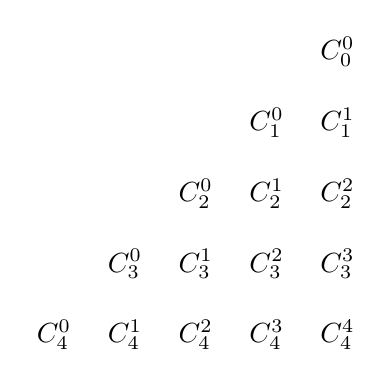
\begin{tikzpicture}[scale=0.9]
    \node[black] at (0,0) {$C_0^0$};
    \node[black] at (-1,-1) {$C_1^0$};
    \node[black] at (0,-1) {$C_1^1$};
    \node[black] at (-2,-2) {$C_2^0$};
    \node[black] at (-1,-2) {$C_2^1$};
    \node[black] at (-0,-2) {$C_2^2$};
    \node[black] at (-3,-3) {$C_3^0$};
    \node[black] at (-2,-3) {$C_3^1$};
    \node[black] at (-1,-3) {$C_3^2$};
    \node[black] at (-0,-3) {$C_3^3$};
    \node[black] at (-4,-4) {$C_4^0$};
    \node[black] at (-3,-4) {$C_4^1$};
    \node[black] at (-2,-4) {$C_4^2$};
    \node[black] at (-1,-4) {$C_4^3$};
    \node[black] at (-0,-4) {$C_4^4$};
\end{tikzpicture}
\hspace{2.5em}
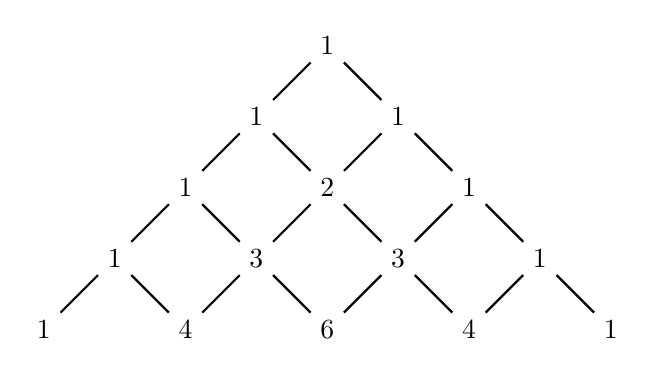
\begin{tikzpicture}[scale=0.9]
    \node[black] (0) at (0,0) {1};
    \node[black] (1) at (-1,-1) {1};
    \node[black] (2) at (1,-1) {1};
    \node[black] (3) at (-2,-2) {1};
    \node[black] (4) at (0,-2) {2};
    \node[black] (5) at (2,-2) {1};
    \node[black] (6) at (-3,-3) {1};
    \node[black] (7) at (-1,-3) {3};
    \node[black] (8) at (1,-3) {3};
    \node[black] (9) at (3,-3) {1};
    \node[black] (10) at (-4,-4) {1};
    \node[black] (11) at (-2,-4) {4};
    \node[black] (12) at (0,-4) {6};
    \node[black] (13) at (2,-4) {4};
    \node[black] (14) at (4,-4) {1};
    \draw[-,thick] (0) to (1);
    \draw[-,thick] (0) to (2);
    \draw[-,thick] (1) to (3);
    \draw[-,thick] (1) to (4);
    \draw[-,thick] (2) to (4);
    \draw[-,thick] (2) to (5);
    \draw[-,thick] (3) to (6);
    \draw[-,thick] (3) to (7);
    \draw[-,thick] (4) to (7);
    \draw[-,thick] (4) to (8);
    \draw[-,thick] (5) to (8);
    \draw[-,thick] (5) to (9);
    \draw[-,thick] (6) to (10);
    \draw[-,thick] (6) to (11);
    \draw[-,thick] (7) to (11);
    \draw[-,thick] (7) to (12);
    \draw[-,thick] (8) to (12);
    \draw[-,thick] (8) to (13);
    \draw[-,thick] (9) to (13);
    \draw[-,thick] (9) to (14);
\end{tikzpicture}

\textbf{例题:}已知函数$y=e^x\cos x$,求$y^{(4)}$。

根据莱布尼兹公式:

$(e^x\cos x)^{(4)}$

$=C_4^0e^x\cos x+C_4^1e^x(-\sin x)+C_4^2e^x(-\cos x)+C_4^3e^x(\sin x)+C_4^4e^x(\cos x)$

$=e^x\cos x+4e^x(-\sin x)+6e^x(-\cos x)+4e^x\sin x+e^x\cos x$

$=-4e^x\cos x$

\section{隐函数与参数方程的导数以及相关变化率}

\subsection{隐函数求导法}

设函数$y=y(x)$由方程$F(x,y)=0$确定的可导函数,则\ding{172}方程两边对自变量$x$求导,($y=y(x)$就是将$y$看作中间变量)得到一个关于$y'$的方程。\ding{173}解该方程就可以得出$y'$。

\textbf{例题:}设$y=y(x)$是由方程$\sin(xy)=\ln\dfrac{x+e}{y}+1$确定的隐函数,求$y'(0)$。

两边求导:

$
\begin{aligned}
    \sin(xy) &=\ln(x+e)-\ln(y)+1 \\
    \cos(xy)(y+xy') &=\dfrac{1}{x+e}-\dfrac{y'}{y} \\
    \because\text{将0代入} & x=0, y=e^2 \\
    e^2&=\dfrac{1}{e}-\dfrac{y'(0)}{e^2} \\
    y'(0) & =e-e^4
\end{aligned}
$

\subsection{参数方程函数导数}

设函数$y=y(x)$由参数方程$\left\{
    \begin{array}{l}
        x=\varphi(t) \\
        y=\psi(t)
    \end{array}
\}\right.$确定,其中$t$为参数,且$\varphi(t)\psi(t)$对于$t$都可导,$\varphi(t)\neq 0$,则:

\medskip

一阶导数:$\dfrac{\rm{d}y}{\rm{d}x}=\dfrac{\rm{d}y/\rm{d}t}{\rm{d}x/\rm{d}t}=\dfrac{\psi'(t)}{\varphi'(t)}=u(t)$。

二阶导数:$\dfrac{\rm{d}^2y}{\rm{d}x^2}=\dfrac{\rm{d}\left(\dfrac{\rm{d}y}{\rm{d}x}\right)}{\rm{d}x}=\dfrac{\rm{d}\left(\dfrac{\rm{d}y}{\rm{d}x}\right)/\rm{d}t}{\rm{d}x/\rm{d}t}=\dfrac{\rm{d}u/\rm{d}t}{\rm{d}x/\rm{d}t}=\dfrac{u'_t}{x'_t}$

\textbf{例题:}设$y=y(x)$由方程$\left\{
\begin{array}{l}
    x=\sin t \\
    y=t\sin t+\cos t
\end{array}
\right.
$($t$为参数)确定,求$\dfrac{\rm{d}^2y}{\rm{d}x^2}\vert_{t=\frac{\pi}{4}}$。

求参数方程的二阶导数首先就要求出其一阶导数:

$\dfrac{\rm{d}y}{\rm{d}x}=\dfrac{y_t'}{x_t'}=\dfrac{t\cos t}{\cos t}=t$。\medskip

$\therefore\dfrac{\rm{d}^2y}{\rm{d}x^2}=\dfrac{\rm{d}\left(\dfrac{\rm{d}y}{\rm{d}x}\right)}{\rm{d}x}=\dfrac{t_t'}{(\sin t)_t'}=\dfrac{1}{\cos t}$\medskip

$\therefore \sqrt{2}$。

当所求是极坐标方程时,可以使用$x=\rho(\theta)\cos\theta$和$y=\rho(\theta)\sin\theta$进行转换为参数方程然后进行求导。

\subsection{相关变化率}

列出依赖于$t$的相关变化率关系式,然后等式两端对$t$求导。

\section{函数微分}

\subsection{定义}

有一个边长为$x$的正方形,变化了$\Delta x$,其面积$\Delta S=(x+\Delta x)^2-x^2=2x\Delta x+(\Delta x)^2$。

当$\Delta x\to 0$时,将这个变化定义为$2x\cdot\Delta x+o(\Delta x)$,前项为线性主部,后面为误差。这个就是$S$的微分。

增量$\Delta y=f(x_0+\Delta)-f(x_0)=A\Delta x+o(\Delta x)$,这个$A\Delta x$定义为$\rm{d}y$,叫做$y$的微分。

$\therefore \rm{d}y\vert_{x=x_0}=A\Delta x=y'(x_0)\cdot\Delta x=y'(x_0)\cdot\rm{d}x$

由此,可导必可微,可微必可导。

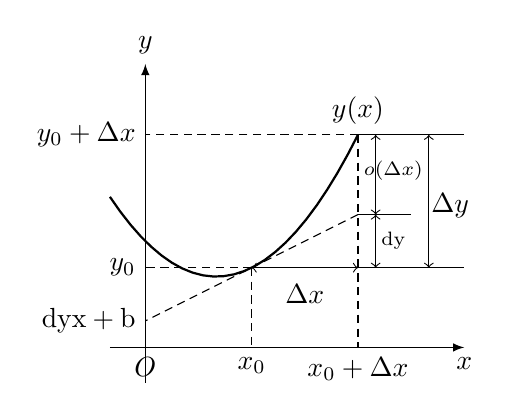
\begin{tikzpicture}[scale=0.9]
    \draw[-latex](-0.5,0) -- (4.5,0) node[below]{$x$};
    \draw[-latex](0,-0.5) -- (0,4) node[above]{$y$};
    \draw[black, thick, domain=-0.5:3] plot (\x,{pow(\x-1,2)/2+1}) node[above]{$y(x)$};
    \filldraw[black] (0,0) node[below]{$O$};
    \draw[black, densely dashed](1.5,1.125) -- (1.5,0) node[below]{$x_0$};
    \draw[black, densely dashed](1.5,1.125) -- (0,1.125) node[left]{$y_0$};
    \draw[black, densely dashed](3,3) -- (3,0) node[below]{$x_0+\Delta x$};
    \draw[black, densely dashed](3,3) -- (0,3) node[left]{$y_0+\Delta x$};
    \draw[black, densely dashed](3,1.875) -- (0,0.375) node[left]{$\rm{d}yx+b$};
    \draw[<->, black](1.5,1.125) -- (3,1.125);
    \draw[<->, black](4,1.125) -- (4,3);
    \draw[<->, black](3.25,1.125) -- (3.25,1.875);
    \draw[<->, black](3.25,3) -- (3.25,1.875);
    \draw[black](3,3) -- (4.5,3);
    \draw[black](3,1.125) -- (4.5,1.125);
    \draw[black](3,1.875) -- (3.75,1.875);
    \filldraw[black] (2.25,0.75) node{$\Delta x$};
    \filldraw[black] (4.3,2) node{$\Delta y$};
    \filldraw[black] (3.5,1.5) node{\scriptsize{$\rm{d}y$}};
    \filldraw[black] (3.5,2.5) node{\scriptsize{$o(\Delta x)$}};
\end{tikzpicture}

所以可微就是用简单线性取代复杂线性,如图用直线取替代曲线。微分就是瞬时改变量,而导数就是瞬时改变速率。

\subsection{基本运算}

\subsubsection{四则运算}

若函数可导:

\begin{enumerate}
    \item 和差的微分:$\rm{d}[u(x)\pm v(x)]=\rm{d}u(x)\pm\rm{d}v(x)$。
    \item 积的微分:$\rm{d}[u(x)v(x)]$$=u(x)\rm{d}v(x)+v(x)\rm{d}u(x)$。
    \item 商的微分:$\rm{d}\left[\dfrac{u(x)}{v(x)}\right]=\dfrac{v(x)\rm{d}u(x)-u(x)\rm{d}v(x)}{[v(x)]^2}$,$v(x)\neq 0$。
    \item 复合函数的微分:链式求导法则$\dfrac{\rm{d}u}{\rm{d}x}=\dfrac{\rm{d}u}{\rm{d}y}\cdot\dfrac{\rm{d}y}{\rm{d}x}$。
\end{enumerate}

\subsubsection{微分形式不变性}

设$y=f(u)$可微,$u=g(x)$可微,则$y=f(g(x))$可微,且$\rm{d}y=y'_x\rm{d}x=y'_u\rm{d}u$。即对哪个变量求导都是一样的,即$\rm{d}\{f[g(x)]\}=f'[g(x)]g'(x)\rm{d}x$。

一阶微分形式不变性指:$\rm{d}f(\varsigma)=f'(\varsigma)\rm{d}\varsigma$,无论$\varsigma$是什么(类似导数的链式求导法则)。

\textbf{例题:}设$y=e^{\sin(\ln x)}$,求$\rm{d}y$。

$\because y=e^{\sin(\ln x)} \therefore$

$
\begin{aligned}
    \rm{d}y &=\rm{d}e^{\sin(\ln x)} \\
    & =e^{\sin(\ln x)}\cdot\rm{d}(\sin(\ln x)) \\
    & =e^{\sin(\ln x)}\cdot\cos(\ln x)\cdot\rm{d}\ln x \\
    & =e^{\sin(\ln x)}\cdot\cos(\ln x)\cdot\dfrac{1}{x}\rm{d}x
\end{aligned}
$

\section{基本求导公式}

\subsection{对幂指函数}

\begin{center}
    \begin{tabular}{|c|c|c|c|}
        \hline
        原函数 & 导函数 & 原函数 & 导函数\\ \hline
        $C$ & $0$ & $n^x$ & $n^x\ln n$ \\ \hline
        $\log_ax$ & $\dfrac{1}{x\ln a}$ & $\ln x=\ln\vert x\vert$ & $\dfrac{1}{x}$ \\ \hline
        $x^n$ & $nx^{n-1}$ & $\sqrt[n]{x}$ & $\dfrac{x^{-\frac{n-1}{n}}}{n}$ \\ \hline
        $\dfrac{1}{x^n}$ & $-\dfrac{n}{x^{n+1}}$ & & \\ 
        \hline
    \end{tabular}
\end{center}

\subsection{三角与反三角函数}

\begin{center}
    \begin{tabular}{|c|c|c|c|}
        \hline
        原函数 & 导函数 & 原函数 & 导函数\\ \hline
        $\sin x$ & $\cos x$ & $\cos x$ & $-\sin x$ \\ \hline
        $\tan x$ & $\dfrac{1}{\cos^2x}=\sec^2x$ & $\cot x$ & $\dfrac{1}{\sin^2x}=\csc^2x$ \\ \hline
        $\sec x$ & $\sec x\tan x$ & $\csc x$ & $-\csc x\cot x$ \\ \hline
        $\arcsin x$ & $\dfrac{1}{1-x^2}$ & $\arccos x$ & $-\dfrac{1}{1-x^2}$ \\ \hline
        $\arctan x$ & $\dfrac{1}{1+x^2}$ & $\rm{arccot}\,\textit{x}$ & $-\dfrac{1}{1+x^2}$ \\ \hline
        $\rm{arcsec}\,\textit{x}$ & $\dfrac{1}{x\sqrt{x^2-1}}$ & $\rm{arccsc}\,\textit{x}$ & $-\dfrac{1}{x\sqrt{x^2-1}}$ \\ \hline
        \hline
    \end{tabular}
\end{center}

\subsection{双曲与反双曲函数}

\begin{itemize}
    \item 双曲正弦:$\rm{sinh}\,\textit{x}=\rm{sh}\,\textit{x}=\dfrac{e^x-e^{-x}}{2}$。
    \item 双曲余弦:$\rm{cosh}\,\textit{x}=\rm{ch}\,\textit{x}=\dfrac{e^x+e^{-x}}{2}$。
    \item 双曲正切:$\rm{tanh}\,\textit{x}=\rm{th}\,\textit{x}=\dfrac{\rm{sinh}\,\textit{x}}{\rm{cosh}\,\textit{x}}=\dfrac{e^x-e^{-x}}{e^x+e^{-x}}$。
    \item 双曲余切:$\rm{coth}\,\textit{x}=\dfrac{\rm{cosh}\,\textit{x}}{\rm{sinh}\,\textit{x}}=\dfrac{e^x+e^{-x}}{e^x-e^{-x}}$。
    \item 双曲正割:$\rm{sech}\,\textit{x}=\dfrac{1}{\rm{cosh}\,\textit{x}}=\dfrac{2}{e^x+e^{-x}}$。
    \item 双曲余割:$\rm{csch}\,\textit{x}=\dfrac{1}{\rm{sinh}\,\textit{x}}=\dfrac{2}{e^x-e^{-x}}$。
    \item 反双曲正弦:$\rm{arcsinh}\,\textit{x}=\ln\left(x+\sqrt{x^2+1}\right)$。
    \item 反双曲余弦:$\rm{arccosh}\,\textit{x}=\ln\left(x+\sqrt{x^2-1}\right)$。
    \item 反双曲正切:$\rm{arctanh}\,\textit{x}=\dfrac{1}{2}\ln\left(\dfrac{1+x}{1-x}\right)$。
\end{itemize}

\begin{center}
    \begin{tabular}{|c|c|c|c|}
        \hline
        原函数 & 导函数 & 原函数 & 导函数\\ \hline
        $\rm{sinh}\,\textit{x}$ & $\rm{cosh}\,\textit{x}$ & $\rm{cosh}\,\textit{x}$ & $\rm{sinh}\,\textit{x}$ \\ \hline
        $\rm{tanh}\,\textit{x}$ & $\dfrac{1}{\rm{cosh}\,\textit{x}^2}$ & $\rm{arcsinh}\,\textit{x}$ & $\dfrac{1}{\sqrt{x^2+1}}$ \\ \hline
        $\rm{arccosh}\,\textit{x}$ & $\dfrac{1}{\sqrt{x^2-1}}$ & $\rm{arctan}\,\textit{x}$ & $\dfrac{1}{1-x^2}$ \\
        \hline
    \end{tabular}
\end{center}

\end{document}
